\chapter{Implementation and Results}
\label{chap:implementation-and-results}

% \input{chapters/out/Implementation and Results.md.tex}

\begin{figure}[H]
  \centering
  \label{fig:simulation-solver-comparison}
  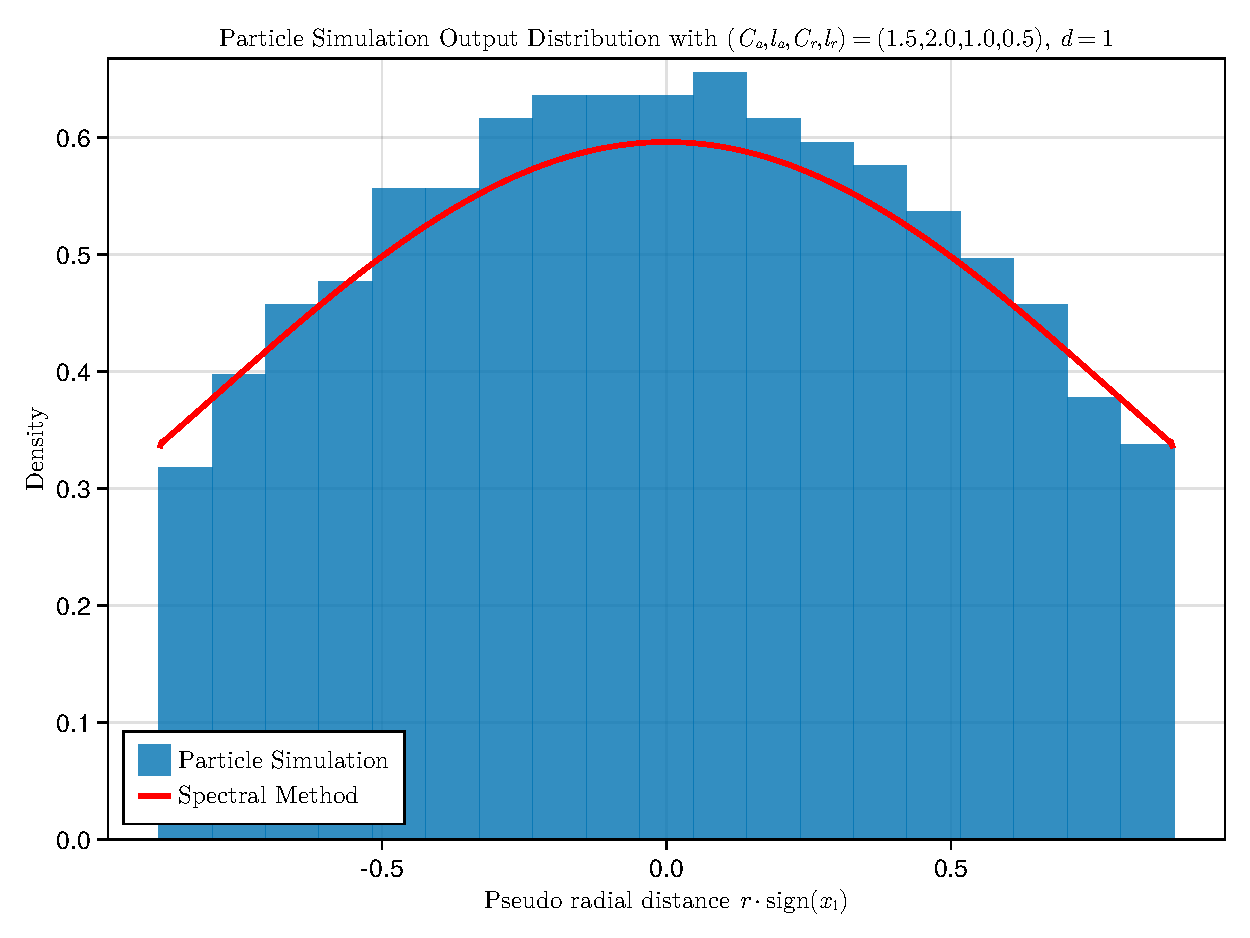
\includegraphics[width=0.8\linewidth]{results/morse/simulation-solver-comparison.pdf}
  \caption[Comparison of histogram and spectral method solution]{Comparison of the radial distance histogram from the simulation output with the $G = 8$ general kernel solvers' equilibrium measure $\rho_{12}(r)$ at $R$ given by the simulator, so without using the outer optimisation routine. The interaction potential in this example is $K(r) = K_{C_a, l_a, C_r, l_r}(r)$ with parameters given above.}
  % for now
\end{figure}

\section{Further Discussion}
\begin{figure}[H]
  \centering
  \label{fig:condition-number-growth}
  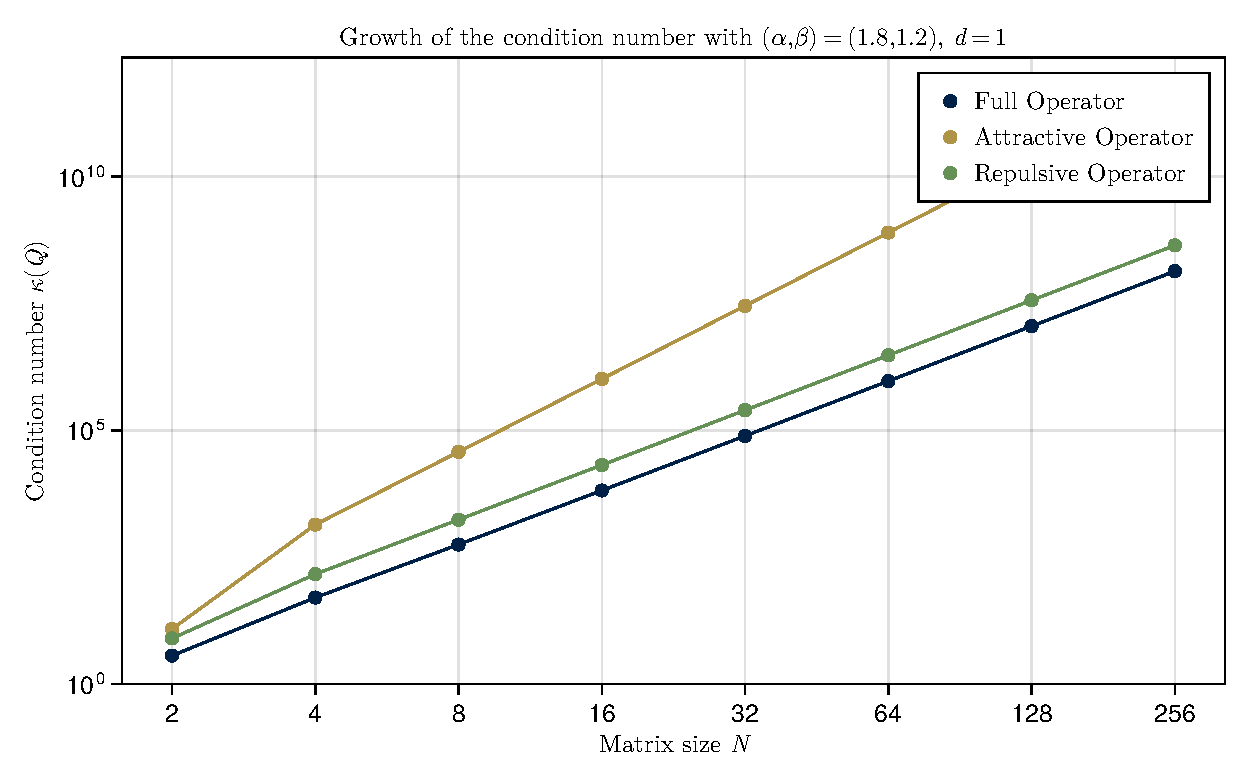
\includegraphics[width=0.8\linewidth]{results/attrep/condition-number-growth.pdf}
  \caption[Growth of the condition number]{Growth of the 2-norm condition number $\kappa(Q)$ of the attractive-repulsive operator $Q$.}
\end{figure}

\begin{figure}[H]
  \centering
  \label{fig:coefficients}
  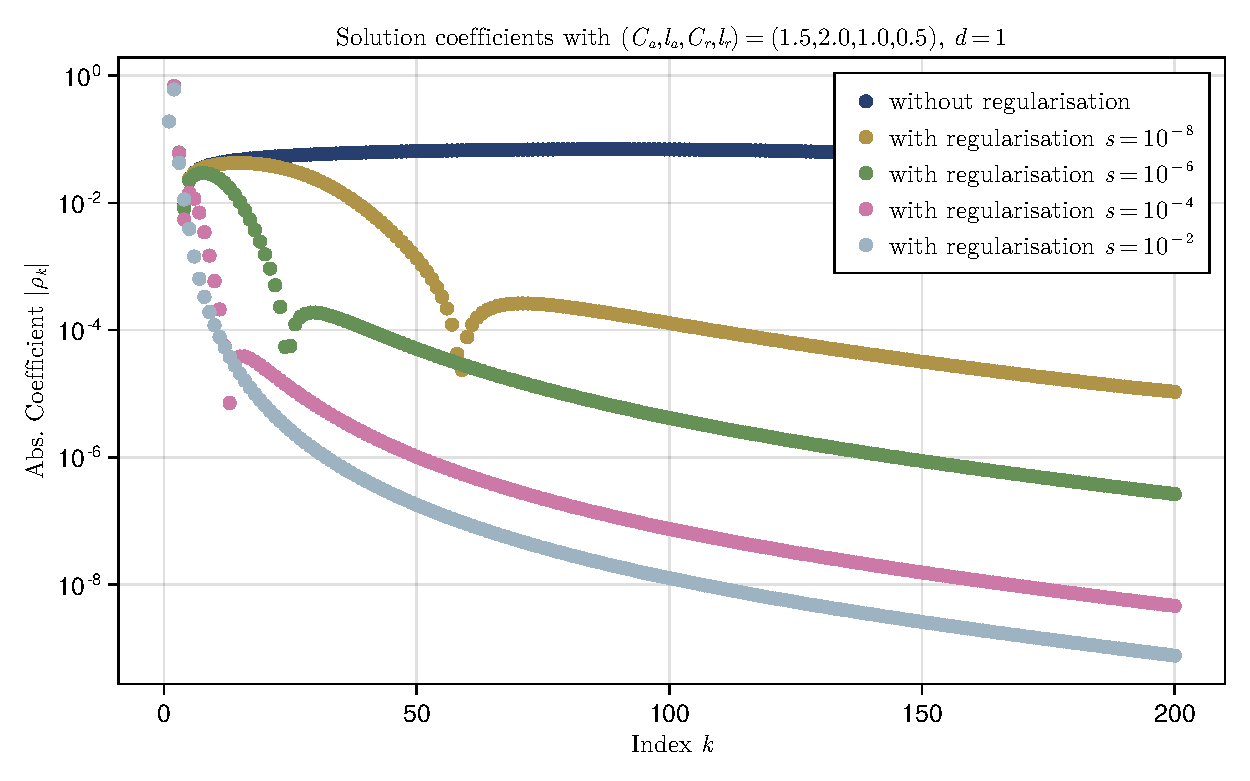
\includegraphics[width=0.8\linewidth]{results/morse/coefficients.pdf}
  \caption[Absolute value of the coefficients with and without regularisation]{Absolute value of the solution coefficients $\rho_k$ with and without Tikhonov regularisation.}
\end{figure}
